\documentclass{article}
\usepackage{graphicx}
\author{Wdataorg}
\date{\today}
\title{The principle of Mja}

\begin{document}
\maketitle
\tableofcontents
\section{Add a sample}
First, \verb|Mja| need least 5 samples to predict


In Mja Software, we use \verb|Add a sample| button to add a 
characteristic information, after input this information, Mja
will convert them into mathematical models


Like this page.
\begin{figure}[htbp]
    \centering
    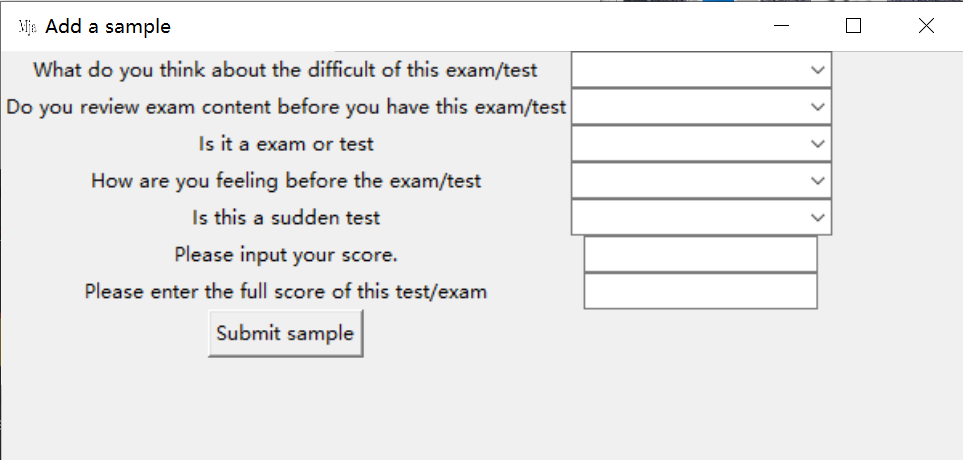
\includegraphics{addsamplepage.png}
\end{figure} 


\subsection{Input sample}
When you have had a exam or test, and you know the score of this exam,
you can use \verb|Add a sample| button to add a information, plenty of information
will make predictions more accurate


If user input all information in this picture, 
they can click this button, Mja will generate a five dimensional model, and save it 
into a file
\subsection{Generate sample group information}
Mja will convert these survey data into a model.How does Mja convert?


Mja will convert each item of data in the survey into a coordinate of the 
five dimensional model 
according to the following table

\begin{tabular}{|c|c|c|c|c|}
\hline
\multicolumn{5}{|c|}{\large Model generation table}
\\\hline
\multicolumn{3}{|c|}{Difficult}
& \multicolumn{2}{|c|}{Have Reviewed}
\\\hline
Easy & Normal & Hard & Have & Haven't \\\hline
1    & 2        & 3  & 1    & 2       \\\hline
\hline
\multicolumn{5}{|c|}{Feeling}\\\hline
Very good & Good & Normal & Bad & Very Bad \\\hline
1 & 2 & 3 & 4 & 5 \\\hline
\hline
\multicolumn{5}{|c|}{Is a Sudden Test}\\\hline
\multicolumn{2}{|c|}{Yes}
& -
& \multicolumn{2}{|c|}{No}\\\hline
\multicolumn{2}{|c|}{1}
& -
& \multicolumn{2}{|c|}{2}\\\hline
\end{tabular}


Such as, user input \verb|Normal|, \verb|Have Reviewed|, 
\verb|Good|, \verb|Yes|, Mja will generate: \verb|[2, 1, 2, 1]|


The last dimension data is the score, 
where the score refers to a ratio. 
For example, if the user 
enters $150$ in the full score 
and $90$ in the score, 
the one-dimensional data 
will be $\frac{90}{150} \times 100$, 
so it is $60$
\subsection{Why do we need least 5 samples?}
When you have no least 5 example, you can not use 
Predict Grades Program, Because Mja Extract the features of the 
first $\sqrt{n}$ samples, When you have only $3$ samples, it will be 
$\sqrt{3} \approx 1$, but Mja uses KNN, KNN need least 2 samples, so 
$n \geq 4$, Because $2^2 = 4$, But to make the results accurate,
so Mja need least 5 samples

\newpage

\section{Calculate with formula}
When we have enough samples, we can 
predict grades, predict grades use cosine 
similarity, It can calculate the cosine of the 
angle between two coordinates,The closer the cosine value is to 1, 
the closer the two vectors are.

Mja used cosine similarity to predict grades.
\subsection{Cosine similarity}
The formula of cosine similarity like this:

\begin{equation}
cos(\theta) = \frac{\sum_{i=1}^{n} (x_i \times y_i)}{{\sqrt{\sum_{i=1}^{n} (x_i)^2}} \times {\sqrt{\sum_{i=1}^{n} (y_i)^2}}}
\end{equation}
\subsection{A example}
I will use a example to tell reader how to use 
this formula


such as we have this data:
\begin{verbatim}
Difficult   Have Reviewed   Feeling     Is a Sudden Test    Score    Full Score
Normal      Have            Good        Yes                 100      150
2           1               2           1                   67       -
\end{verbatim}

and we have this new list
\begin{verbatim}
3           1               2           2                   70       -
\end{verbatim}

Substitute into this formula

\begin{equation}
cos(\theta) = \frac{2 \times 3 + 
1 \times 1 + 2 \times 2 + 1 \times 2}{\sqrt{2^2
+ 1^2 + 2^2 + 1^2} \times \sqrt{3^2 + 1^2 + 2^2 +2^2}}
 \approx 0.97
\end{equation}

So we can they these samples are very close
\subsection{Sort cosine similarity list}
First, we should use this formula to 
calculate the similarity of samples to
 be tested and all known samples. And then sort them 


For example, we have similarity list:
\verb|[(0.998, 90), (0.678, 80), (0.892, 95), (0.977, 100)]|


After sort them, we can get the new similarity list:
\verb|[(0.998, 90), (0.977, 100), (0.892, 95), (0.678, 80)]|

\subsection{Delete samples with low similarity}
Then, we have a sorted list.


We only need first $\sqrt{list. length()}$ elements


Such as, similarity list:\verb|[(0.998, 90), (0.977, 100), (0.892, 95), (0.678, 80)]|
$\sqrt{list.length()} = 2$, so we only need
\verb|[(0.998, 90), (0.977, 1000)]|

\subsection{Regression}
At last, we should \textbf{Regression} similarity list.


This step only requires the average similarity value


The value of similarity list \verb|[(0.998, 90), (0.977, 1000)]| is
\verb|[90, 100]|, average it, we can get the results
$95$.


Congratulations, you successfully completed the result forecast!
\end{document}